%Define useful lengths
\newlength{\boxwidth}
\setlength{\boxwidth}{2cm}
\newlength{\boxheight}
\setlength{\boxheight}{1.5cm}
\newlength{\boxdepthx}
\setlength{\boxdepthx}{0.5\boxwidth}
\newlength{\boxdepthy}
\setlength{\boxdepthy}{0.5\boxheight}

%Define useful positions w/short-hand notation
%pos-position, b-bottom, t-top, l-left, r-right, f-front, d-distant
\newcommand\posbfl{(-\boxwidth,-\boxheight)}
\newcommand\posbfr{(\boxwidth,-\boxheight)}
\newcommand\posbdr{(\boxwidth+\boxdepthx,-\boxheight+\boxdepthy)}
\newcommand\posbdl{(-\boxwidth+\boxdepthx,-\boxheight+\boxdepthy)}
\newcommand\postfl{(-\boxwidth,\boxheight)}
\newcommand\postfr{(\boxwidth,\boxheight)}
\newcommand\postdr{(\boxwidth+\boxdepthx,\boxheight+\boxdepthy)}
\newcommand\postdl{(-\boxwidth+\boxdepthx,\boxheight+\boxdepthy)}

\centering
\begin{tikzpicture}
  %insert galaxy-image in center
  \node (galaxy) at (0.5\boxdepthx,0.5\boxdepthy) {\includegraphics[width=\boxwidth]{../tikzfigures/galaxy_thumbnail/galaxy.png}};
  %draw bottom plate
  \draw \posbfl -- \posbfr -- \posbdr -- \posbdl -- \posbfl;
  %draw top plate
  \draw \postfl -- \postfr -- \postdr -- \postdl -- \postfl;
  %draw vertical connectors
  \draw \posbfl -- \postfl;
  \draw \posbfr -- \postfr;
  \draw \posbdl -- \postdl;
  \draw \posbdr -- \postdr;
  %add inflow above box
  \draw[thick,->] (0,1.5\boxheight+\boxdepthy) -- (0,1.2\boxheight+\boxdepthy);
  %\draw (-0.5\boxdepthx,2\boxheight) -- (0,2\boxheight-0.5\boxdepthx) -- (0.5\boxdepthx,2\boxheight);
  %\draw (-0.25\boxdepthx,3\boxheight) -- (-0.25\boxdepthx,2\boxheight);
  %\draw (0.25\boxdepthx,3\boxheight) -- (0.25\boxdepthx,2\boxheight);
  \node at (0.6\boxwidth, 1.3\boxheight+\boxdepthy) {\small Primordial gas};
  %add outflow below box
  \draw[thick,->] (0,-1.2\boxheight) -- (0,-1.5\boxheight);
  %\draw (-0.5\boxdepthx,-2\boxheight) -- (0,-2\boxheight-0.5\boxdepthx) -- (0.5\boxdepthx,-2\boxheight);
  %\draw (-0.25\boxdepthx,-1\boxheight) -- (-0.25\boxdepthx,-2\boxheight);
  %\draw (0.25\boxdepthx,-1\boxheight) -- (0.25\boxdepthx,-2\boxheight);
  \node at (0.6\boxwidth, -1.3\boxheight) {\small Enriched gas};
\end{tikzpicture}
\caption[Diagram inflow/outflow one-zone galaxy model]{\label{tikz:galaxy-iobox}
The diagram shows the concept of inflow and outflow of a one-zone galaxy model.
All gas content is initially prestine (from big bang nucleosynthesis), as is the gas content of the extragalactic medium.
Star formation in the galaxy synthesized heavy metals and enriches the gas content of the galaxy. Star formation is also a major contributing to supernovae, which in turn drive outflow of enriched material into the extragalactic medium.
This does not mean that any enriched material is returned from the extragalactic medium, that would require a two-zone galaxy model.
}
